\documentclass[12pt]{article}
\linespread{1.2}
\usepackage{graphicx} % Required for inserting images
\usepackage{tabularray}
\UseTblrLibrary{tikz,functional,amsmath}
\usepackage{indentfirst}
\usepackage{amsmath,amsthm,amssymb,graphicx,upgreek}
\usepackage{amsmath,mathtools}
\usepackage{bm}
\usepackage{float} % For [H] float placement
\usepackage[colorlinks,linkcolor=black,]{hyperref}
\usepackage{xeCJK}
\usepackage[top=2cm, bottom=2cm, left=2cm, right=2cm, a4paper]{geometry}
\setCJKmainfont{FandolKai}
\newtheorem{theorem}{Theorem}[section]
\newtheorem{corollary}{Corollary}[section]
\newtheorem{axiom}{Axiom}[section]
\newtheorem{definition}{Definition}[section]
\newtheorem{proposition}{Proposition}[section]
\newtheorem{lemma}{Lemma}[section]
\newtheorem{application}{Application}[section]
\newtheorem{inference}{Inference}[section]
\newcommand{\de}[1]{\mathrm{d}#1}
\newcommand{\mrm}[1]{\mathrm{#1}}
\newcommand{\mbf}[1]{\mathbf{#1}}
\newcommand{\bb}[1]{\mathbb{#1}}
\newcommand{\ca}[1]{\mathcal{#1}}
\newcommand{\dd}[1]{\frac{\mathrm{d}}{\mathrm{d}#1}}
\newcommand{\kh}[1]{\left(#1\right)}
\newcommand{\zkh}[1]{\left[#1\right]}
\newcommand{\dkh}[1]{\left.#1\right\}}
\newcommand{\dkhz}[1]{\left\{#1\right.}
\newcommand{\sh}[1]{^{#1}}
\newcommand{\xia}[1]{_{#1}}
\newcommand{\ed}[1]{\(\rm{(end)}\)}
\newcommand{\blue}[1]{\textcolor{blue}{#1}}
\newcommand{\red}[1]{\color{red}{#1}}
\usepackage{xcolor}

% 定义新颜色
\definecolor{red}{RGB}{255,0,0}
\definecolor{blue}{HTML}{0000FF}
\definecolor{green}{cmyk}{1,0,1,0}

\title{Methods of Mathematical Physics A\\Assignment 3}
\author{H.R. Yu}
\date{March 2026}

\begin{document}

\maketitle

\section{}
\subsection{}
\subsubsection{}
\begin{align*}
\int_{0}^{2+\mathrm{i}} \mathrm{Re}\,z\,\mathrm{d}z &= \int_{0}^{2} \mathrm{Re}\,z\,\mathrm{d}z + \int_{2}^{2+\mathrm{i}} \mathrm{Re}\,z\,\mathrm{d}z \\
&= \int_0^2 x\de x+\int_0^{1}2\mrm i \de y\\
&= \frac{1}{2} \times 2^2 + 2 \mrm i \\
&= 2+2 \mrm i.
\end{align*}
\subsubsection{}
\begin{align*}
\int_{0}^{2+\mathrm{i}} \mathrm{Re}\,z\,\mathrm{d}z &= (2+\mathrm{i}) \int_{0}^{1} 2t\,\mathrm{d}t \\
&= 2+\mathrm{i}.
\end{align*}
\subsection{}
\subsubsection{}
\begin{align*}
\int_{C} \frac{\mathrm{d}z}{\sqrt{z}} &= \int_{0}^{\pi} \mathrm{i}\,\mathrm{e}^{\mathrm{i}\frac{\theta}{2}} \mathrm{d}\theta \\
&= \left. 2\mathrm{e}^{\mathrm{i}\frac{\theta}{2}} \right\vert_{0}^{\pi} \\
&= 2\mathrm{e}^{\mathrm{i}\frac{\pi}{2}} - 2 \\
&= 2(\mathrm{i} - 1).
\end{align*}
\subsubsection{}
\begin{align*}
\int_{C} \frac{\mathrm{d}z}{\sqrt{z}} &= \int_{0}^{-\pi} \mathrm{i}\,\mathrm{e}^{\mathrm{i}\frac{\theta}{2}} \mathrm{d}\theta \\
&= \left. 2\mathrm{e}^{\mathrm{i}\frac{\theta}{2}} \right\vert_{0}^{-\pi} \\
&= 2\mathrm{e}^{-\mathrm{i}\frac{\pi}{2}} - 2 \\
&= -2(1+\mathrm{i}).
\end{align*}
\section{}
\subsection{}
\subsubsection{}
$\frac{\sin \frac{\pi z}{4}}{z^2 - 1}$ 在 $C: \vert z \vert = \frac{1}{2}$ 包围的单连通区域内解析，故由$\mathrm{Cauchy}$定理，
\begin{align*}
\oint_{C} \frac{1}{z^2 - 1} \sin \frac{\pi z}{4} \,\mathrm{d}z = 0.
\end{align*}
\subsubsection{}
记\[f(z) = \frac{\sin \frac{\pi z}{4}}{z+1},\]$f(z)$ 在 $C: \vert z - 1 \vert = 1$ 包围的单连通区域内解析，由$\mathrm{Cauchy}$积分公式
\begin{align*}
f(a) = \frac{1}{2\pi \mathrm{i}} \oint_{C} \frac{f(z)}{z - a} \,\mathrm{d}z,
\end{align*}
得
\begin{align*}
\oint_{C} \frac{1}{z^2 - 1} \sin \frac{\pi z}{4} \,\mathrm{d}z&=\oint_{C} \frac{f(z)}{z - 1} \,\mathrm{d}z \\
&= 2\pi \mathrm{i} f(1) \\
&= \mathrm{i} \frac{\sqrt{2}}{2} \pi.
\end{align*}
\subsubsection{}
用割线\([-3\mrm i, 3\mrm i]\)将积分路径切为两个半圆，记\[f(z) = \frac{\sin \frac{\pi z}{4}}{z+1}, \quad g(z) = \frac{\sin \frac{\pi z}{4}}{z-1},\]
则由Cauchy积分公式得
\begin{align*}
\oint_{C_1} \frac{f(z)}{z - 1} \,\mathrm{d}z &= 2\pi \mathrm{i} f(1) \\
&= \mathrm{i} \frac{\sqrt{2}}{2} \pi, \\
\oint_{C_2} \frac{g(z)}{z + 1} \,\mathrm{d}z &= 2\pi \mathrm{i} g(-1) \\
&= \mathrm{i} \frac{\sqrt{2}}{2} \pi,
\end{align*}
故
\begin{align*}
\oint_{C} \frac{1}{z^2 - 1} \sin \frac{\pi z}{4} \,\mathrm{d}z &= \oint_{C_1} \frac{f(z)}{z - 1} \,\mathrm{d}z + \oint_{C_2} \frac{g(z)}{z + 1} \,\mathrm{d}z \\
&= \mathrm{i} \sqrt{2} \pi.
\end{align*}
\subsubsection{}
沿虚轴用割线将积分路径切为两个半圆，记\[f(z) = \frac{\sin \frac{\pi z}{4}}{z+1}, \quad g(z) = \frac{\sin \frac{\pi z}{4}}{z-1},\]
结果同上一问，两条路径各包含一个奇点，由Cauchy积分公式得
\begin{align*}
\oint_{C} \frac{1}{z^2 - 1} \sin \frac{\pi z}{4} \,\mathrm{d}z &= \oint_{C_1} \frac{f(z)}{z - 1} \,\mathrm{d}z + \oint_{C_2} \frac{g(z)}{z + 1} \,\mathrm{d}z \\
&= \mathrm{i} \sqrt{2} \pi.
\end{align*}
\subsection{}
\subsubsection{}
记\[f(z) = \frac{\mathrm{e}^{\mathrm{i} z}}{z + \mathrm{i}},\]$f(z)$ 在路径 $C: \vert z - \mathrm{i} \vert = 1$ 包围的单连通区域内解析，故由$\mathrm{Cauchy}$积分公式得
\begin{align*}
\oint_{C} \frac{1}{z^2 + 1} \mathrm{e}^{\mathrm{i} z} \,\mathrm{d}z &= \oint_{C} \frac{f(z)}{z - \mathrm{i}} \,\mathrm{d}z \\
&= 2\pi \mathrm{i} f(\mathrm{i}) \\
&= \frac{\pi}{\mathrm{e}}.
\end{align*}
\subsubsection{}
用割线 $[-2, 2]$ 切割积分路径，记\[f(z) = \frac{\mathrm{e}^{\mathrm{i} z}}{z + \mathrm{i}},\quad g(z) = \frac{\mathrm{e}^{\mathrm{i} z}}{z - \mathrm{i}},\]
由$\mathrm{Cauchy}$积分公式得
\begin{align*}
\oint_{C} \frac{\mathrm{e}^{\mathrm{i} z}}{z^2 + 1} \,\mathrm{d}z &= \oint_{C_1} \frac{f(z)}{z - \mathrm{i}} \,\mathrm{d}z + \oint_{C_2} \frac{g(z)}{z + \mathrm{i}} \,\mathrm{d}z \\
&= 2\pi \mathrm{i} f(\mathrm{i}) + 2\pi \mathrm{i} g(-\mathrm{i}) \\
&= \frac{\pi}{\mathrm{e}} - \pi \mathrm{e}.
\end{align*}
\subsubsection{}
用割线 $[- 1, 1]$ 切割积分路径，记\[f(z) = \frac{\mathrm{e}^{\mathrm{i} z}}{z + \mathrm{i}},\quad g(z) = \frac{\mathrm{e}^{\mathrm{i} z}}{z - \mathrm{i}},\]
同上一问，两个半椭圆连通区域各含一个奇点，由$\mathrm{Cauchy}$积分公式得
\begin{align*}
\oint_{C} \frac{\mathrm{e}^{\mathrm{i} z}}{z^2 + 1} \,\mathrm{d}z &= \oint_{C_1} \frac{f(z)}{z - \mathrm{i}} \,\mathrm{d}z + \oint_{C_2} \frac{g(z)}{z + \mathrm{i}} \,\mathrm{d}z \\
&= 2\pi \mathrm{i} f(\mathrm{i}) + 2\pi \mathrm{i} g(-\mathrm{i}) \\
&= \frac{\pi}{\mathrm{e}} - \pi \mathrm{e}.
\end{align*}
\subsubsection{}
作图：
\begin{figure}[H]
    \centering
    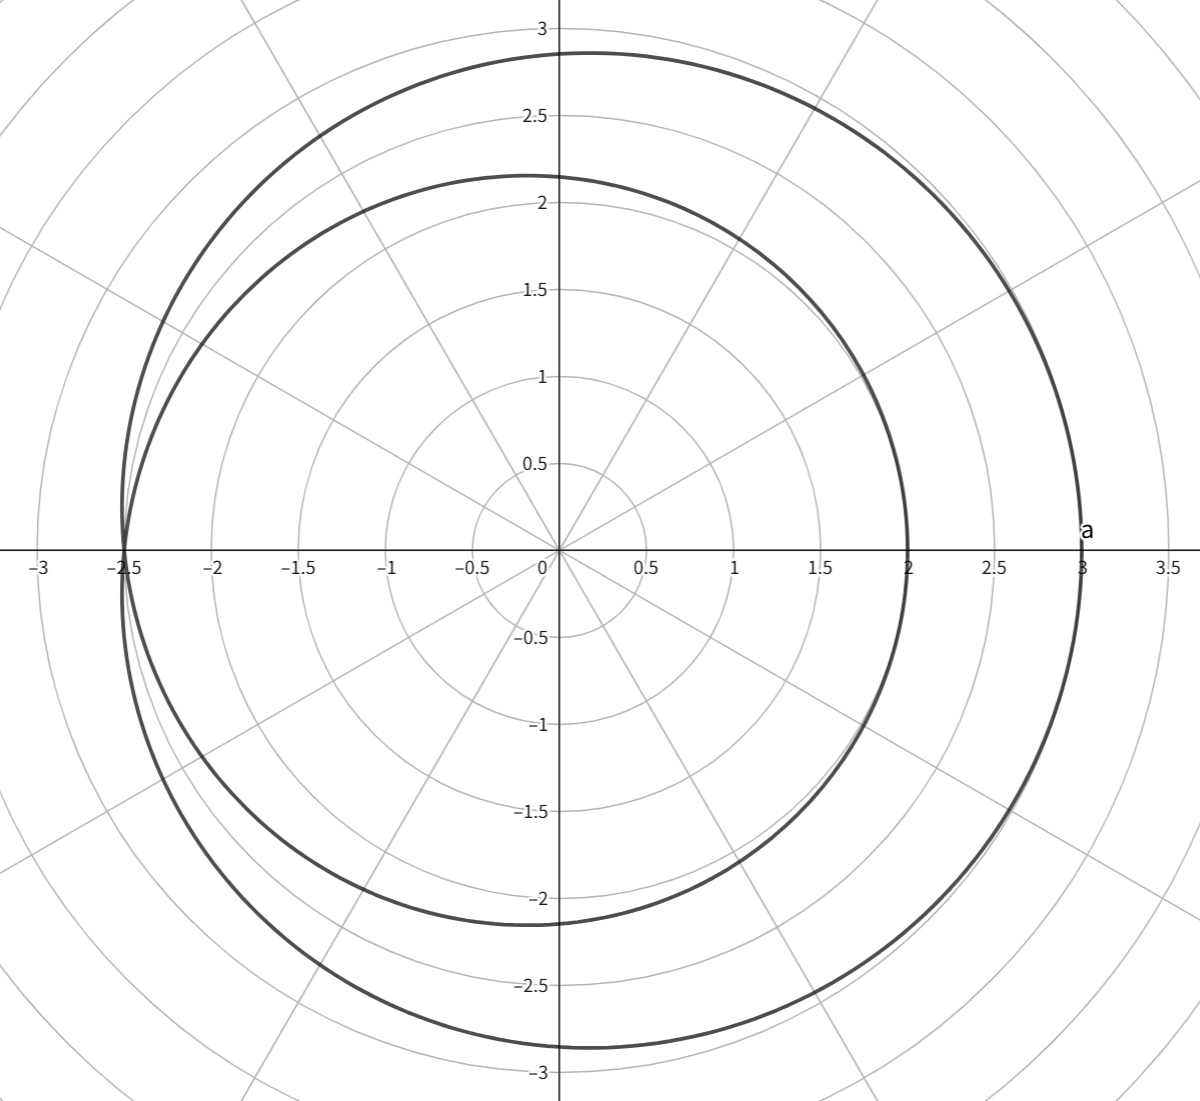
\includegraphics[width=0.45\linewidth]{p1.png}
\end{figure}
积分路径可以分成两条闭合曲线，每条闭合曲线都包含了两个奇点. 对每个闭合曲线，用割线切割，再应用Cauchy积分公式得
\begin{align*}
    \oint_{C} \frac{\mathrm{e}^{\mathrm{i} z}}{z^2 + 1} \,\mathrm{d}z &= \oint_{C_a} \frac{\mathrm{e}^{\mathrm{i} z}}{z^2 + 1} \,\mathrm{d}z + \oint_{C_b} \frac{\mathrm{e}^{\mathrm{i} z}}{z^2 + 1} \,\mathrm{d}z\\
    &=\oint_{C_{a1}} \frac{f(z)}{z - \mathrm{i}} \,\mathrm{d}z +\oint_{C_{a2}} \frac{g(z)}{z + \mathrm{i}} \,\mathrm{d}z+\oint_{C_{b1}} \frac{f(z)}{z - \mathrm{i}} \,\mathrm{d}z+ \oint_{C_{b2}} \frac{g(z)}{z + \mathrm{i}} \,\mathrm{d}z \\
    &= 2\times 2\pi \mathrm{i} f(\mathrm{i}) + 2\times 2\pi \mathrm{i} g(-\mathrm{i}) \\
    &= 2\kh{\frac{\pi}{\mathrm{e}} - \pi \mathrm{e}}.
\end{align*}
\section{}
\begin{proof}
记积分
\begin{align*}
    I&=\int_0^\pi \mrm e^{\cos\theta}\cos\kh{\sin\theta}\de \theta\\
    &=\frac{1}{2}\times\int_0^\pi \kh{\mrm e^{\cos \theta+\mrm i\sin \theta}+\mrm e^{\cos \theta-\mrm i\sin \theta}}\de \theta\\
    &=\frac{1}{2}\times\int_0^\pi \kh{\mrm e^{\mrm e^{\mrm i\theta}}+\mrm e^{\mrm e^{-\mrm i\theta}}}\de \theta,
\end{align*}
记\[w=\mrm e^{\mrm i \theta},\; u=\mrm e^{-\mrm i\theta},\]
则
\begin{align*}
    I&=-\frac{\mrm i}{2}\times \kh{\int_0^{\mrm e^{\mrm i\pi}}\frac{1}{w}\mrm e^w\de w-\int_0^{\mrm e^{-\mrm i\pi}}\frac{1}{u}\mrm e^u\de u}\\
    &=-\frac{\mrm i}{2}\times \int_{\mrm e^{-\mrm i\pi}}^{\mrm e^{\mrm i\pi}}\frac{1}{w}\mrm e^w\de w.
\end{align*}

计算
\begin{align*}
    \oint_{|z|=1}\frac{\mrm e^z}{z}\de z,
\end{align*}
由Cauchy积分公式
\begin{align*}
    f\kh{a}=\frac{1}{2\pi \mrm i}\oint_C \frac{f\kh{z}}{z-a}\de z,
\end{align*}
于是
\begin{align*}
    \oint_{|z|=1}\frac{\mrm e^z}{z}\de z&=2\pi \mrm i \mrm e^0\\
    &=2\pi \mrm i.
\end{align*}

代入原积分得
\begin{align*}
    I&=-\frac{\mrm i}{2}\times \int_{\mrm e^{-\mrm i\pi}}^{\mrm e^{\mrm i\pi}}\frac{1}{w}\mrm e^w\de w\\
    &=-\frac{\mrm i}{2}\times \oint_{|w|=1}\frac{1}{w}\mrm e^w\de w\\
    &=-\frac{\mrm i}{2}\times 2\pi \mrm i\\
    &=\pi.
\end{align*}
\end{proof}
\section{}
\subsection{}
记
\[
f(z) = \frac{\ln(z+3)}{z^2+5},
\]
在 $C$ 包围的单连通区域内，$f(z)$ 解析. 由 Cauchy 积分公式得
\begin{align*}
\oint_C \frac{\ln(z+3)}{z(z^2+5)} \mathrm{d}z &= \oint_C \frac{f(z)}{z-0} \mathrm{d}z \\
&= 2\pi\mathrm{i} \cdot f(0) \\
&= \mathrm{i} \frac{2\pi\ln 3}{5}.
\end{align*}
\subsection{}
奇点 $(0,0)$ 在 $C$ 包围的单连通区域内，
记 $f(z) = \mathrm{e}^{-z}\sin(2z)$，则
\[
f'(z) = \left(2\cos 2z - \sin 2z\right)\mathrm{e}^{-z}.
\]
$f(z)$ 在$C$包围的单连通区域内解析，由导数 Cauchy 积分公式
\[
f^{(n)}(z) = \frac{n!}{2\pi\mathrm{i}} \oint_C \frac{f(w)}{(w-z)^{n+1}} \mathrm{d}w,
\]
得
\begin{align*}
f'(a) &= \frac{1}{2\pi\mathrm{i}} \oint_C \frac{f(z)}{(z-a)^2} \mathrm{d}z.
\end{align*}
令 $a=0$，得
\begin{align*}
\oint_C \frac{\mathrm{e}^{-z}\sin(2z)}{z^2} \mathrm{d}z &= \oint_C \frac{f(z)}{z^2} \mathrm{d}z \\
&= 2\pi\mathrm{i} f'(0) \\
&= 4\pi\mathrm{i}.
\end{align*}
\subsection{}
奇点 $(0,1),(0,-1)$ 均在 $C$ 包围的单连通区域内，
用割线 $[-2,2]$ 将积分路径切为两个半圆 $C_1,C_2$. 
记
\[
f(z) = \frac{z^2-1}{z+i}, \quad g(z) = \frac{z^2-1}{z-i},
\]
$f(z)$ 在 $C_1$ 内解析，$g(z)$ 在 $C_2$ 内解析. 由 Cauchy 积分公式得
\begin{align*}
\oint_C \frac{z^2-1}{z^2+1} \mathrm{d}z &= \oint_{C_1} \frac{f(z)}{z-i} \mathrm{d}z + \oint_{C_2} \frac{g(z)}{z+i} \mathrm{d}z \\
&= 2\pi\mathrm{i} f(i) + 2\pi\mathrm{i} g(-i) \\
&= 0.
\end{align*}
\subsection{}
当 \( n \in \mathbb{N} \) 时，\( \left( z-a \right)^n \) 在 \( C \) 内解析，由 Cauchy 定理，
\begin{align*}
\oint_C \left( z-a \right)^n \mathrm{d}z = 0.
\end{align*}

当 \( n \in \mathbb{Z}^- /\{-1\}\) 时，奇点 \( z=a \) 在 \( C \) 内，由导数 Cauchy 积分公式
\begin{align*}
f^{(n)}(z) = \frac{n!}{2\pi\mathrm{i}} \oint_C \frac{f(w)}{\left( w-z \right)^{n+1}} \mathrm{d}w,
\end{align*}
故
\begin{align*}
\oint_C \frac{\mathrm{d}z}{\left( z-a \right)^{-n}} &= \frac{2\pi\mathrm{i}}{(-n-1)!} f^{(-n-1)}(a),
\end{align*}
其中 \( f(z) = 1 \).

故\( f^{(-n-1)}(a) = 0 \)，从而
\begin{align*}
\oint_C \left( z-a \right)^n \mathrm{d}z = 0.
\end{align*}

若 \( n = -1 \)，则
\begin{align*}
\oint_C \frac{\mathrm{d}z}{z-a} &= 2\pi\mathrm{i} f(a) \\
&= 2\pi\mathrm{i}.
\end{align*}

综上，
\begin{align*}
\oint_C \left( z-a \right)^n \mathrm{d}z =
\begin{cases}
0, & n \neq -1, \\
2\pi\mathrm{i}, & n = -1.
\end{cases}
\end{align*}
\subsection{}
奇点 \( (1,0),(2,0) \) 均在 \( C \) 内，
记
\[
f(z) = \frac{\sin\left( \pi z \right) + \cos\left( \pi z^2 \right)}{z-1}, \quad g(z) = \frac{\sin\left( \pi z \right) + \cos\left( \pi z^2 \right)}{z-2},
\]
\( f(z) \) 在 \( C_1 \) 内解析，\( g(z) \) 在 \( C_2 \) 内解析，由 Cauchy 积分公式得
\begin{align*}
\oint_C \frac{\sin\left( \pi z \right) + \cos\left( \pi z^2 \right)}{\left( z-1 \right)\left( z-2 \right)} \mathrm{d}z &= \oint_{C_1} \frac{f(z)}{z-2} \mathrm{d}z + \oint_{C_2} \frac{g(z)}{z-1} \mathrm{d}z \\
&= 2\pi\mathrm{i} f(2) + 2\pi\mathrm{i} g(1) \\
&= 2\pi\mathrm{i} + 2\pi\mathrm{i} \\
&= 4\pi\mathrm{i}.
\end{align*}
\subsection{}
在 \( C \) 上 \( z \neq 0 \)，且恒有 \( \vert z \vert = 8 \)，从而
\begin{align*}
\oint_C \frac{\overline{z}}{z^2 - \overline{z}} \mathrm{d}z &= \oint_C \frac{z\overline{z}}{z^3 - z\overline{z}} \mathrm{d}z \\
&= \oint_C \frac{\vert z \vert^2}{z^3 - \vert z \vert^2} \mathrm{d}z \\
&= \oint_C \frac{64}{z^3 - 64} \mathrm{d}z \\
&= 64 \times \oint_C \frac{1}{z^3 - 4^3} \mathrm{d}z.
\end{align*}

\( C \) 内有 3 个奇点 \( z=4 \)，\( 4\mathrm{e}^{\mathrm{i}\frac{2}{3}\pi} \)，\( 4\mathrm{e}^{\mathrm{i}\frac{4}{3}\pi} \).

用割线将 \( C \) 切为 3 个\(\frac{1}{3}\)圆 \( C_1,C_2,C_3 \)，记
\[
f(z) = \frac{1}{\left( z-4\mathrm{e}^{\mathrm{i}\frac{2}{3}\pi} \right)\left( z-4\mathrm{e}^{\mathrm{i}\frac{4}{3}\pi} \right)}, \quad
g(z) = \frac{1}{\left( z-4 \right)\left( z-4\mathrm{e}^{\mathrm{i}\frac{4}{3}\pi} \right)}, \quad
h(z) = \frac{1}{\left( z-4 \right)\left( z-4\mathrm{e}^{\mathrm{i}\frac{2}{3}\pi} \right)},
\]
则
\begin{align*}
\oint_C \frac{\overline{z}}{z^2 - \overline{z}} \mathrm{d}z
&= 64 \times \oint_C \frac{1}{z^3 - 4^3} \mathrm{d}z \\
&= 64 \times \left( \oint_{C_1} \frac{f(z)}{z-4} \mathrm{d}z + \oint_{C_2} \frac{g(z)}{z-4\mathrm{e}^{\mathrm{i}\frac{2}{3}\pi}} \mathrm{d}z + \oint_{C_3} \frac{h(z)}{z-4\mathrm{e}^{\mathrm{i}\frac{4}{3}\pi}} \mathrm{d}z \right) \\
&= 64 \times \left[ 2\pi\mathrm{i} f(4) + 2\pi\mathrm{i} g\left( 4\mathrm{e}^{\mathrm{i}\frac{2}{3}\pi} \right) + 2\pi\mathrm{i} h\left( 4\mathrm{e}^{\mathrm{i}\frac{4}{3}\pi} \right) \right] \\
&= 128\pi\mathrm{i} \left[ f(4) + g\left( 4\mathrm{e}^{\mathrm{i}\frac{2}{3}\pi} \right) + h\left( 4\mathrm{e}^{\mathrm{i}\frac{4}{3}\pi} \right) \right] \\
&= 8\pi\mathrm{i} \times \left( 3 -\frac{3}{2} - \frac{3 \sqrt{3}}{2}\mathrm{i} - \frac{3}{2} + \frac{3 \sqrt{3}}{2}\mathrm{i} \right) \\
&= 0.
\end{align*}
\end{document}
